\documentclass{beamer}

\usepackage{amsmath}
\usepackage{mathtools}

\usepackage{tikz}
\usetikzlibrary{arrows}
\usepackage{xcolor}
\makeatletter


\def\pgfpathgrid{\pgfutil@ifnextchar[{\pgf@pathgrid}{\pgf@pathgrid[]}}
\def\pgf@pathgrid[#1]#2#3{%
  \pgfset{#1}%
  \pgfmathsetlength\pgf@xc{\pgfkeysvalueof{/pgf/stepx}}%
  \pgfmathsetlength\pgf@yc{\pgfkeysvalueof{/pgf/stepy}}%
  \pgf@process{#3}%
  \pgf@xb=\pgf@x%
  \pgf@yb=\pgf@y%
  \pgf@process{#2}%
  \pgf@xa=\pgf@x\relax%
  \pgf@ya=\pgf@y\relax%
  {%
    % compute bounding box
    % first corner
    \pgf@x=\pgf@xb%
    \pgf@y=\pgf@yb%
    \pgf@pos@transform{\pgf@x}{\pgf@y}%
    \pgf@protocolsizes{\pgf@x}{\pgf@y}%
    % second corner
    \pgf@x=\pgf@xb%
    \pgf@y=\pgf@ya%
    \pgf@pos@transform{\pgf@x}{\pgf@y}%
    \pgf@protocolsizes{\pgf@x}{\pgf@y}%
    % third corner
    \pgf@x=\pgf@xa%
    \pgf@y=\pgf@yb%
    \pgf@pos@transform{\pgf@x}{\pgf@y}%
    \pgf@protocolsizes{\pgf@x}{\pgf@y}%
    % fourth corner
    \pgf@x=\pgf@xa%
    \pgf@y=\pgf@ya%
    \pgf@pos@transform{\pgf@x}{\pgf@y}%
    \pgf@protocolsizes{\pgf@x}{\pgf@y}%
  }%
  \c@pgf@counta=\pgf@y\relax% Truncate the start y coordinate to integer
  \c@pgf@countb=\pgf@yc\relax% Truncate the step size to integer
  \divide\c@pgf@counta by\c@pgf@countb\relax% Truncate the ratio
  \pgf@y=\c@pgf@counta\pgf@yc\relax% % Find the closest integer-multiple of step size to the start
    \ifdim\pgf@ya>\pgf@yb% If the start point is larger than finish 
        \c@pgf@counta=-1\relax
    \else % If everything is fine
        \c@pgf@counta=1\relax
    \fi
  \ifdim\the\c@pgf@counta\pgf@y<\the\c@pgf@counta\pgf@ya% If for some reason it goes too far
    \advance\pgf@y by\the\c@pgf@counta\pgf@yc% take back one step size
  \fi%
  \loop% horizontal lines
    {%
      \pgf@xa=\pgf@x%
      \pgf@ya=\pgf@y%
      \pgf@pos@transform{\pgf@xa}{\pgf@ya}
      \pgfsyssoftpath@moveto{\the\pgf@xa}{\the\pgf@ya}%
      \pgf@xa=\pgf@xb%
      \pgf@ya=\pgf@y%
      \pgf@pos@transform{\pgf@xa}{\pgf@ya}
      \pgfsyssoftpath@lineto{\the\pgf@xa}{\the\pgf@ya}%
    }%
    \advance\pgf@y by\the\c@pgf@counta\pgf@yc% Increment in the - or + direction
  \ifdim\the\c@pgf@counta\pgf@y<\the\c@pgf@counta\pgf@yb% Also compare with the correct sign.
  \repeat%
  \advance\pgf@y by 0.01\dimexpr0pt-(1pt)*\c@pgf@counta\relax%
  \ifdim\the\c@pgf@counta\pgf@y<\the\c@pgf@counta\pgf@yb
    {%
      \pgf@xa=\pgf@x%
      \pgf@ya=\pgf@y%
      \pgf@pos@transform{\pgf@xa}{\pgf@ya}
      \pgfsyssoftpath@moveto{\the\pgf@xa}{\the\pgf@ya}%
      \pgf@xa=\pgf@xb%
      \pgf@ya=\pgf@y%
      \pgf@pos@transform{\pgf@xa}{\pgf@ya}
      \pgfsyssoftpath@lineto{\the\pgf@xa}{\the\pgf@ya}%
    }%
  \fi%
  \c@pgf@counta=\pgf@x\relax%
  \c@pgf@countb=\pgf@xc\relax%
  \divide\c@pgf@counta by\c@pgf@countb\relax%
  \pgf@x=\c@pgf@counta\pgf@xc\relax%
    \ifdim\pgf@xa>\pgf@xb% If the start point is larger than finish 
      \c@pgf@counta=-1\relax
    \else % If everything is fine
      \c@pgf@counta=1\relax
    \fi
  \ifdim\the\c@pgf@counta\pgf@x<\the\c@pgf@counta\pgf@xa%
    \advance\pgf@x by\the\c@pgf@counta\pgf@xc%
  \fi%
  \loop% vertical lines
    {%
      \pgf@xc=\pgf@x%
      \pgf@yc=\pgf@ya%
      \pgf@pos@transform{\pgf@xc}{\pgf@yc}
      \pgfsyssoftpath@moveto{\the\pgf@xc}{\the\pgf@yc}%
      \pgf@xc=\pgf@x%
      \pgf@yc=\pgf@yb%
      \pgf@pos@transform{\pgf@xc}{\pgf@yc}
      \pgfsyssoftpath@lineto{\the\pgf@xc}{\the\pgf@yc}%
    }%
    \advance\pgf@x by\the\c@pgf@counta\pgf@xc% Increment in the - or + direction
  \ifdim\the\c@pgf@counta\pgf@x<\the\c@pgf@counta\pgf@xb% Also compare with the correct sign.
  \repeat%
  \advance\pgf@x by 0.01\dimexpr0pt-(1pt)*\c@pgf@counta\relax%
  \ifdim\the\c@pgf@counta\pgf@x<\the\c@pgf@counta\pgf@xb%
    {%
      \pgf@xc=\pgf@x%
      \pgf@yc=\pgf@ya%
      \pgf@pos@transform{\pgf@xc}{\pgf@yc}
      \pgfsyssoftpath@moveto{\the\pgf@xc}{\the\pgf@yc}%
      \pgf@xc=\pgf@x%
      \pgf@yc=\pgf@yb%
      \pgf@pos@transform{\pgf@xc}{\pgf@yc}
      \pgfsyssoftpath@lineto{\the\pgf@xc}{\the\pgf@yc}%
    }%
  \fi%
}


\makeatother

\newcommand{\arrow}[2]{\draw[->,blue,thick,shorten <=5mm, shorten >=5mm] #1 -- #2 ;}


\usetheme{Madrid}

\usepackage{booktabs}
\usepackage{subcaption}

\title[Physician Scheduling]{Physician Scheduling in a Gynaecology Department}
\subtitle{MSc Dissertation}
\author{S.T.~Luen-English}
\institute[Cardiff University]
{
  Department of Mathematics\\
  Cardiff University}

\date{September 2015}

\AtBeginSection[]
{
  \begin{frame}<beamer>{Outline}
    \tableofcontents[currentsection,currentsubsection]
  \end{frame}
}

\begin{document}

\begin{frame}
  \titlepage
\end{frame}

\begin{frame}{Outline}
\setcounter{tocdepth}{1}
  \tableofcontents
  % You might wish to add the option [pausesections]
\end{frame}

\section{Introduction}

\begin{frame}{Introduction}
    \begin{figure}
        \centering
        \includegraphics[width=0.6\linewidth]{img/utwente}
        \caption{University of Twente, Enschede}
    \end{figure}
\end{frame}

\begin{frame}{Introduction}
    \begin{figure}
        \centering
        %http://www.limburgia.nl/Files/PhotoAlbum/13455522474680120508-03-664.jpg
        \begin{subfigure}{.45\textwidth}
            \centering
            \includegraphics[width=\linewidth]{img/hospital1}
            \caption{}
        \end{subfigure}
        \hfill
        %http://www.egm.nl/uploads/projecten/afbeeldingen/Jeroen-Bosch-Ziekenhuis-EGM-architecten-37.jpg
        \begin{subfigure}{.45\textwidth}
            \centering
            \includegraphics[width=\linewidth]{img/hospital2}
            \caption{}
        \end{subfigure}
        \caption{Jeroen Bosch Ziekenhuis}
    \end{figure}
\end{frame}

\begin{frame}{Introduction}
    \begin{itemize}
        \item Personnel scheduling problem found in the Gynaecology Department in Jeroen Bosch Hospital, 's-Hertogenbosch
        \item Problem of timetabling doctors: specifying both what shifts they work, but also what task they will be doing in that shift
        \item Currently done by hand, taking 2-3 days to schedule the next 6 weeks
    \end{itemize}
\end{frame}

\section{Problem Description}
\begin{frame}{Introduction}
    \center
    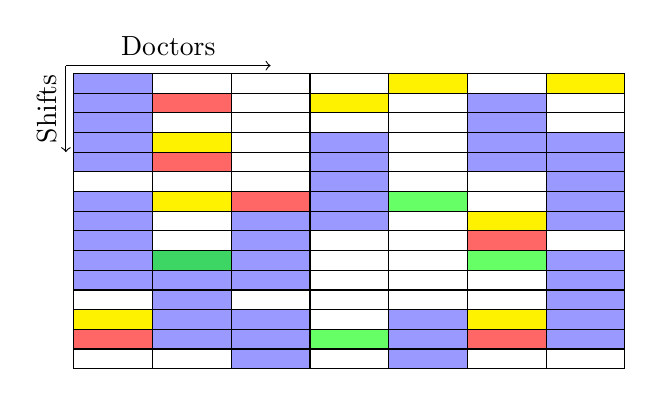
\begin{tikzpicture}[scale =0.5]
        \draw[->] (-0.2,0.2) -- (5,0.2) node [midway, above] (TextNode) {Doctors};
        \draw[<-] (-0.2,-2) -- (-0.2,0.2)node [midway, above, sloped] (TextNode) {Shifts};
        \foreach \x/\y in {0/0, 6/-1.5, 0/-3, 2/-4.5, 12/-1.5, 12/-4.5}{
        \fill[blue,opacity=.4] (\x, \y) rectangle (\x+2,\y-2.5);}
        \foreach \x/\y in {4/-3.5, 10/-0.5}{
        \fill[blue,opacity=.4] (\x, \y) rectangle (\x+2,\y-2);}
        \foreach \x/\y in {4/-6, 8/-6}{
        \fill[blue,opacity=.4] (\x, \y) rectangle (\x+2,\y-1.5);}
        \foreach \x/\y in {0/-6.5, 2/-0.5, 2/-2, 4/-3, 10/-4, 10/-6.5}{
        \fill[red, opacity=.6] (\x, \y) rectangle (\x+2,\y-.5);}
        \foreach \x/\y in {0/-6, 2/-1.5, 2/-3, 6/-0.5, 8/0, 10/-3.5, 10/-6, 12/0}{
        \fill[yellow, opacity=1] (\x, \y) rectangle (\x+2,\y-.5);}
        \foreach \x/\y in {2/-4.5, 6/-6.5, 8/-3, 10/-4.5}{
        \fill[green, opacity=.6] (\x, \y) rectangle (\x+2,\y-.5);}
        \draw[xstep=2cm, ystep=0.5cm,black,thin] (0,0) grid (14,-7.5);
    \end{tikzpicture}
    \begin{itemize}
        \item Both essential and desired properties that a schedule must meet
            \begin{itemize}
                \item Relating to individual doctors work patterns e.g. days off, contracted hours, `fair' proportion of undesirable tasks etc...
                \item Relating to overall scheduling of task e.g. adequate clinics scheduled each month, always two doctors on-call etc...
            \end{itemize}
    \end{itemize}
\end{frame}

\begin{frame}{Similar Problems}
    \begin{itemize}
        \item Nurse Rostering Problem
        \item (Master) Physician Scheduling Problem
        \item Employee Timetabling Problem
    \end{itemize}
\end{frame}

\section{Mixed Integer Linear Program}

\begin{frame}{Introduction}
    \begin{itemize}
        \item General linear program formulation:
            %
            \begin{equation*}
                \begin{aligned}
                    \text{Min} \quad \mathbf{c}^T \mathbf{x} \\
                    \text{s.t.} \quad
                    \mathbf{A}\mathbf{x} \geq \mathbf{b} \\
                    \mathbf{x \geq 0}
                \end{aligned}
            \end{equation*}
            %
        \item Decision variable:
            %
            \begin{equation*}\begin{gathered}
                x_{i,j,s,t} = 
                \begin{cases}
                    1 & \text{if doctor $i$ does task $t$ on shift $s$ on day $j$} \\
                    0 & \text{otherwise}
                \end{cases}
            \end{gathered}\end{equation*}
            %
        \item Can easily express problem in terms `hard' and `soft' constraints; for example:
            %
            \begin{equation*}
                \sum_{t \in T} x_{i,j,s,t} \leq 1 \quad \forall\; i \in I, j \in J, s \in S
            \end{equation*}
            %
            To ensure a doctor can only be assigned to one task per shift
    \end{itemize}
\end{frame}

\begin{frame}{Objective Function}
    Weighted sum of soft constraint violations, for example:
    \begin{itemize}
        \item Under-scheduling of tasks weekly
        \item Under and over scheduling of each doctor with respect to contract:
        \item Instances when a doctor has `holes' in schedule
        \item Tasks being unfairly distributed among doctors
    \end{itemize}
\end{frame}

\begin{frame}{Solution Progress}
    \begin{figure}
        \centering
        \includegraphics[width=0.75\textwidth]{img/Base2MIPclose}
        \caption{8 Week Planning Horizon: Solution Progress}
    \end{figure}
\end{frame}

\section{Local Search Framework}

\begin{frame}{Local Search Framework}
    \begin{itemize}
        \item Starting from some initial solution, repeatedly attempt to improve solution through some small change
        \item Move operators:
            \begin{itemize}
                \item Schedule task
                \item Delete scheduled task
                \item Swap 2 shift assignments in a week
                \item Change doctor performing a on-call sequence
                \item Swap between doctors performing on-call tasks
            \end{itemize}
    \end{itemize}
\end{frame}

\begin{frame}{Move Operators}
    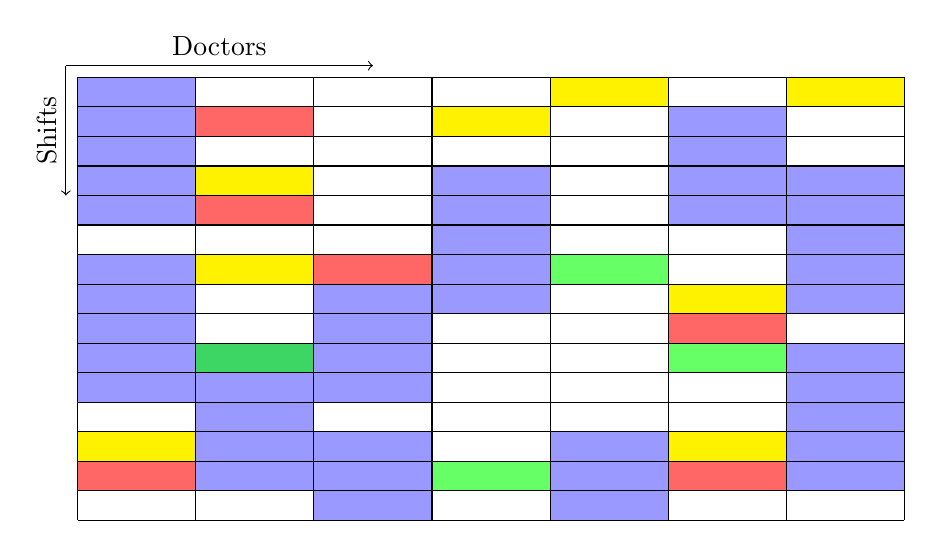
\begin{tikzpicture}[scale =0.75]
        \draw[->] (-0.2,0.2) -- (5,0.2) node [midway, above] (TextNode) {Doctors};
        \draw[<-] (-0.2,-2) -- (-0.2,0.2)node [midway, above, sloped] (TextNode) {Shifts};
        \foreach \x/\y in {0/0, 6/-1.5, 0/-3, 2/-4.5, 12/-1.5, 12/-4.5}{
        \fill[blue,opacity=.4] (\x, \y) rectangle (\x+2,\y-2.5);}
        \foreach \x/\y in {4/-3.5, 10/-0.5}{
        \fill[blue,opacity=.4] (\x, \y) rectangle (\x+2,\y-2);}
        \foreach \x/\y in {4/-6, 8/-6}{
        \fill[blue,opacity=.4] (\x, \y) rectangle (\x+2,\y-1.5);}
        \foreach \x/\y in {0/-6.5, 2/-0.5, 2/-2, 4/-3, 10/-4, 10/-6.5}{
        \fill[red, opacity=.6] (\x, \y) rectangle (\x+2,\y-.5);}
        \foreach \x/\y in {0/-6, 2/-1.5, 2/-3, 6/-0.5, 8/0, 10/-3.5, 10/-6, 12/0}{
        \fill[yellow, opacity=1] (\x, \y) rectangle (\x+2,\y-.5);}
        \foreach \x/\y in {2/-4.5, 6/-6.5, 8/-3, 10/-4.5}{
        \fill[green, opacity=.6] (\x, \y) rectangle (\x+2,\y-.5);}
        \draw[xstep=2cm, ystep=0.5cm,black,thin] (0,0) grid (14,-7.5);
    \end{tikzpicture}
\end{frame}

\begin{frame}{Simulated Annealing}
    \begin{itemize}
        \item Local search likely to get stuck in `local optimum'
        \item Simulated annealing aims to overcome this by probabilistic acceptance of worsening moves
            \begin{itemize}
                \item At beginning of search, high probability of accepting worsening moves
                \item Probability decreases as search continues
            \end{itemize}
    \end{itemize}
\end{frame}

\begin{frame}{Implementation}
    \begin{itemize}
        \item Mixed Integer Linear Program implemented in AIMMS 4.6 and solved using CPLEX 12.6
        \item Repeated Local Search and Simulated Annealing where implemented in Python programming language
            \begin{itemize}
                \item Repeated Local Search ran multiple search processes simultaneously over multiple CPU cores
            \end{itemize}
    \end{itemize}
\end{frame}

\section{Results}
\begin{frame}{Results}
    \begin{table}[H]
        \centering
        \caption{Results Summary}
        \label{fig:results}
        \begin{tabular}{cccccccccc}
            \toprule
            & \multicolumn{3}{c}{\textbf{4 Week}} & \multicolumn{3}{c}{\textbf{8 Week}} & \multicolumn{3}{c}{\textbf{12 Week}} \\
            \cmidrule(lr){2-4}\cmidrule(lr){5-7}\cmidrule(lr){8-10}
            \textbf{Case}      & \textbf{MIP}       & \textbf{SA}       & \textbf{RLS}      & \textbf{MIP}           & \textbf{SA}           & \textbf{RLS}          & \textbf{MIP}           & \textbf{SA}           & \textbf{RLS}          \\
            \cmidrule(lr){1-1}\cmidrule(lr){2-4}\cmidrule(lr){5-7}\cmidrule(lr){8-10}
            0         & 1386      & 1476     & 1490     & 2203          & 2393         & 2380         & 114411        & 3393         & 3365         \\
            1         & 1336      & 1376     & 1441     & 2136          & 2249         & 2401         & 2938          & 3493         & 3273         \\
            2         & 1322      & 1483     & 1501     & 2123          & 2486         & 2454         & 110421        & 3351         & 3458        \\
            3         & 1358      & 1525     & 1489     & 2383          & 2502         & 2512         & 105894        & 3508         & 3411         \\ \bottomrule
        \end{tabular}
    \end{table}
\end{frame}

\begin{frame}{Remarks}
    \begin{itemize}
        \item In almost all cases the MIP was the best performer
        \item Local search algorithms could be improved through the use of `faster' programming language
        \item Quantification of solutions is subjective; is beneficial to give decision maker a choice of `good solutions': something local search algorithms can do well
    \end{itemize}
\end{frame}


\begin{frame}{The End}
    \begin{center}
        Thanks for listening! \\
        \vspace{12pt}
        Luen-EnglishST@cardiff.ac.uk
    \end{center}
\end{frame}
\end{document}
